\subsection{String Matching}

\begin{frame}[fragile] 
  \frametitle{String Matching}
  String matching algorithms are an important class of string algorithms that try
  to find a place where one string (also called pattern) are found within a larger
  string or text.
  \vspace{3mm}
  \begin{itemize}
  \item Naive
  \item Boyer Moore
  \end{itemize}
\end{frame}

\begin{frame}[fragile] 
  \frametitle{Naive}
  Align the pattern at the beginning of the text and compare each character.
  Move the character one position to the right in case of a mismatch!\\
  \vspace{3mm}
  {\small
  \verb|T: GCTTCTGCTACCTTTTGCGCGCGCGCGGAA|\\
  \verb|P: CCTTTTGC|\\
  \verb|    CCTTTTGC|\\
  \verb|     CCTTTTGC|\\
  \verb|      CCTTTTGC|\\
  \verb|       CCTTTTGC|\\
  \verb|        ...|\\
  \verb|             CCTTTTGC|\\
  }
\end{frame}

\begin{frame}[fragile] 
  \frametitle{Boyer Moore}
  This algorithm will use the knowledge from the character comparisons to skip
  future alignments that will definitly not match.\\
  {\bf Start to scan the pattern from the right side!}\\
  In case of a mismatch we can skip comparisons in case the character in the text
  doesn’t happen to appear in the pattern.
\end{frame}

\begin{frame}[fragile]
  \frametitle{Boyer Moore}
  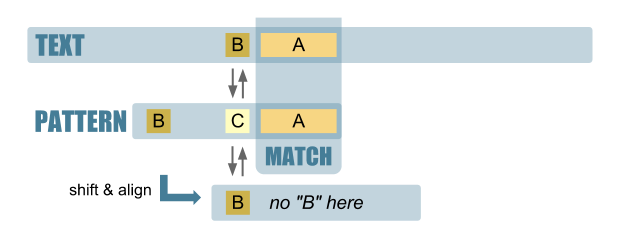
\includegraphics[scale=0.4]{img/bm1.png}\\
  \vspace{1mm}
  The mismatched character B from the text appears in the beginning of the pattern.
  Therefore the pattern will be shifted to the right until character B in the
  pattern and text are aligend.
\end{frame}

\begin{frame}[fragile]
  \frametitle{Boyer Moore}
  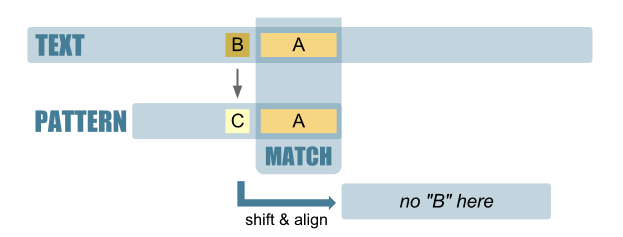
\includegraphics[scale=0.4]{img/bm2.png}\\
  \vspace{1mm}
  If the mismatched character B is not contained in the pattern, then the whole
  pattern can be shifted forward.
\end{frame}

\begin{frame}[fragile] 
\frametitle{Boyer Moore - Example}
\verb|T: er sagte abrakadabra aber|\\
\verb|P: aber|\\
\verb|       aber|\\
\verb|        aber|\\
\verb|            aber|\\
\verb|               aber|\\
\verb|                   aber|\\
\verb|                      aber|\\
\verb|                        aber|
\end{frame}

\begin{frame}[fragile]
\frametitle{Edit Distance}
The edit distance is a way of quantifying how dissimilar two strings are to one another by counting the minimum number of operations (insert, delete, substitue) required to transform one string into the other.\\
\vspace{3mm}
If a user types \emph{graffe}? What could he mean?
\begin{itemize}
\item graf
\item graft
\item grail
\item giraffe
\end{itemize}

\end{frame}

\begin{frame}[fragile]
\frametitle{Edit Distance - Example}
\verb|I N T E * N T I O N|\\
\verb|' ' ' ' ' ' ' ' ' '|\\
\verb|* E X E C U T I O N|\\
 
\vspace{3mm}

The editing distance is 5.\\
3 Substitutions + 2 Insertions\\

\vspace{3mm}

\begin{exercise}
What is the minimum editing distance of \emph{GUMBO} and \emph{GAMBOL}?
\end{exercise}

\end{frame}

\begin{frame}[fragile]
\frametitle{Edit Distance}
Two string s and t are given.\\
$m = length(s)$\\
$n = length(t)$\\
\vspace{3mm}
Initialize\\
$D_{0,0} = 0$\\
$D_{i,0} = i, 1 \leq i \leq m$\\
$D_{0,j} = j, 1 \leq j \leq n$
\end{frame}

\begin{frame}[fragile]
\frametitle{Edit Distance}
\begin{tabular}{|c|c|c|c|c|c|c|}
\hline
 & & G & U & M & B & O\\
\hline
 & 0 & 1 & 2 & 3 & 4 & 5\\
\hline
G & 1 & & & & &\\
\hline
A & 2 & & & & &\\
\hline
M & 3 & & & & &\\
\hline
B & 4 & & & & &\\
\hline
O & 5 & & & & &\\
\hline
L & 6 & & & & &\\
\hline
\end{tabular}
\end{frame}

\begin{frame}[fragile]
\frametitle{Edit Distance}
Calculate each cell with the following formula:
\begin{align}
D_{i,j}= min \left\{
\begin{aligned} & D_{i-1,j-1} + 0 & & t_i = s_i\\
& D_{i-1,j-1} + 1 & & t_i \neq s_i (Substitute)\\
& D_{i,j-1} + 1 & & (Insert)\\
& D_{i-1,j} + 1 & & (Delete)\\
\end{aligned}\right.
\end{align}
\end{frame}

\begin{frame}[fragile]
\frametitle{Edit Distance}
\begin{tabular}{|c|c|c|c|c|c|c|}
\hline
 & & G & U & M & B & O\\
\hline
 & 0 & 1 & 2 & 3 & 4 & 5\\
\hline
G & 1 & 0 & 1 & 2 & 3 & 4\\
\hline
A & 2 & 1 & 1 & 2 & 3 & 4\\
\hline
M & 3 & 2 & 2 & 1 & 2 & 3\\
\hline
B & 4 & 3 & 3 & 2 & 1 & 2\\
\hline
O & 5 & 4 & 4 & 3 & 2 & 1\\
\hline
L & 6 & 5 & 5 & 4 & 3 & {\bf 2}\\
\hline
\end{tabular}\\
\vspace{3mm}
The final result is in the lower right hand corner!
\end{frame}

